\subsection{Opgave 33}

Figuren viser grafen for et andengradspolynomium f.

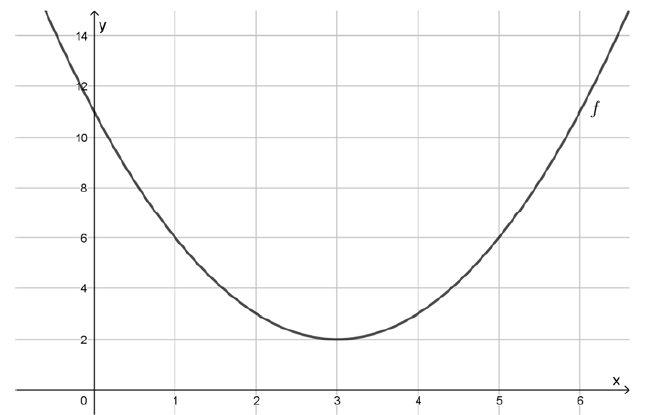
\includegraphics[width=8cm]{Opgave_31-40/Opgave_33/33.png}

Benyt grafen til at løse ligningen $f(x) = 6$

\ans

For at løse ligningen $f(x) = 6$ skal vi altså finde de steder funktionen har en y værdi på 6, og derefter aflæse de tilhørende x værdier.

Jeg tegner en vandret linje der går igennem $y = 6$ og aflæser x værdierne til de steder hvor den vandrette linje skærer funktionen f.

Jeg få de 2 x værdier og dermed de 2 løsninger $x = 1$ og $x = 5$.

Løsningerne er illustreret på nedenstående figur.

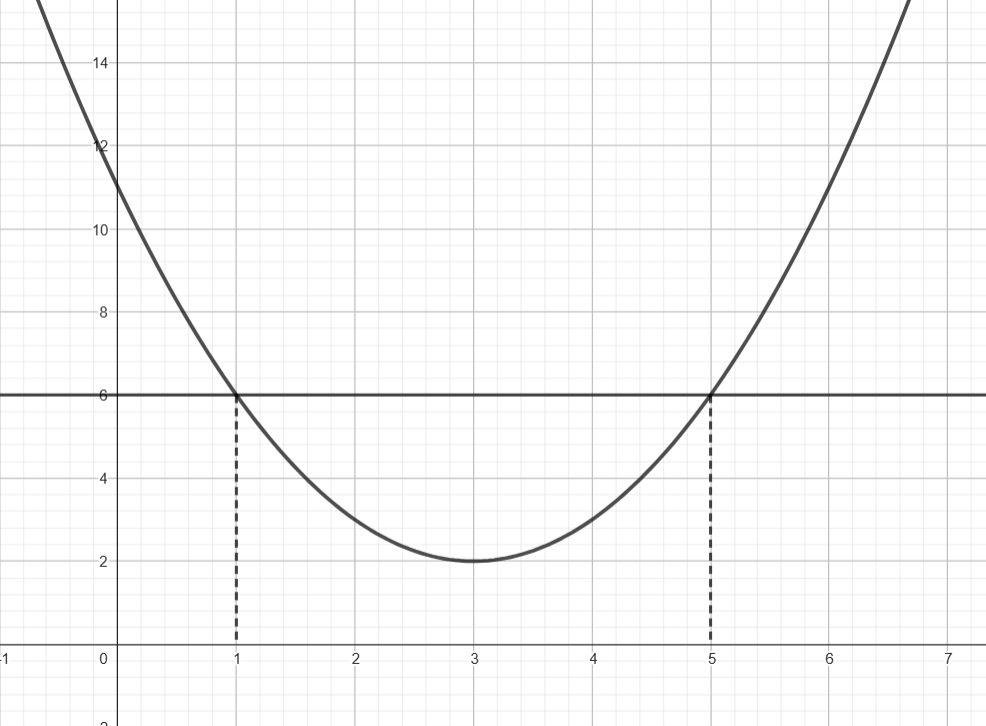
\includegraphics[width=8cm]{Opgave_31-40/Opgave_33/33.1.png}